\section{Domain Policies}
\label{app:domain-policies}

\subsection{Verified Airline and Retail policies}

\subsubsection{Retail policy}
\label{app:retail-policy}
\inputminted[escapeinside=||, fontsize=\small, breaklines, breaksymbol=, breaksymbolleft=, breaksymbolright=, breakanywhere, bgcolor=blue!5]{markdown}{codes/retail_agent_policy.md}

\subsubsection{Airline policy}
\label{app:airline-policy}
\inputminted[escapeinside=||, fontsize=\small, breaklines, breaksymbol=, breaksymbolleft=, breaksymbolright=, breakanywhere, bgcolor=green!5]{markdown}{codes/airline_agent_policy.md}

\subsection{Telecom policy}
\label{app:telecom-policy}

Telecom policy is composed of two parts:
\begin{itemize}
    \item Generic policy \Cref{app:generic-telecom-policy}
    \item Technical support policy (default and workflow) \Cref{app:technical-support-policy,app:technical-support-policy-workflow}
\end{itemize}

\subsubsection{Generic telecom policy}
\label{app:generic-telecom-policy}


\inputminted[escapeinside=||, fontsize=\small, breaklines, breaksymbol=, breaksymbolleft=, breaksymbolright=, breakanywhere, bgcolor=purple!5]{markdown}{codes/telecom_agent_generic.md}

\subsubsection{Technical support policy (original)}
\label{app:technical-support-policy}

\inputminted[escapeinside=||, fontsize=\small, breaklines, breaksymbol=, breaksymbolleft=, breaksymbolright=, breakanywhere, bgcolor=purple!5]{markdown}{codes/telecom_agent_troubleshooting.md}

In \solomode mode, the agent is provided with a version of those policies that have been rephrased when needed.
(e.g instructions like "ask user to do X", are rephrased as "perform action X")


\subsubsection{Technical support policy (workflow)}
\label{app:technical-support-policy-workflow}

\inputminted[escapeinside=||, fontsize=\small, breaklines, breaksymbol=, breaksymbolleft=, breaksymbolright=, breakanywhere, bgcolor=purple!5]{markdown}{codes/telecom_agent_troubleshooting.md}

\subsubsection{Troubleshooting workflow graphs}
\label{app:troubleshooting-workflow-graphs}

To help the agent understand the troubleshooting workflow, we provide a decision graph for each issue type.

\begin{figure}[htbp]
    \centering
    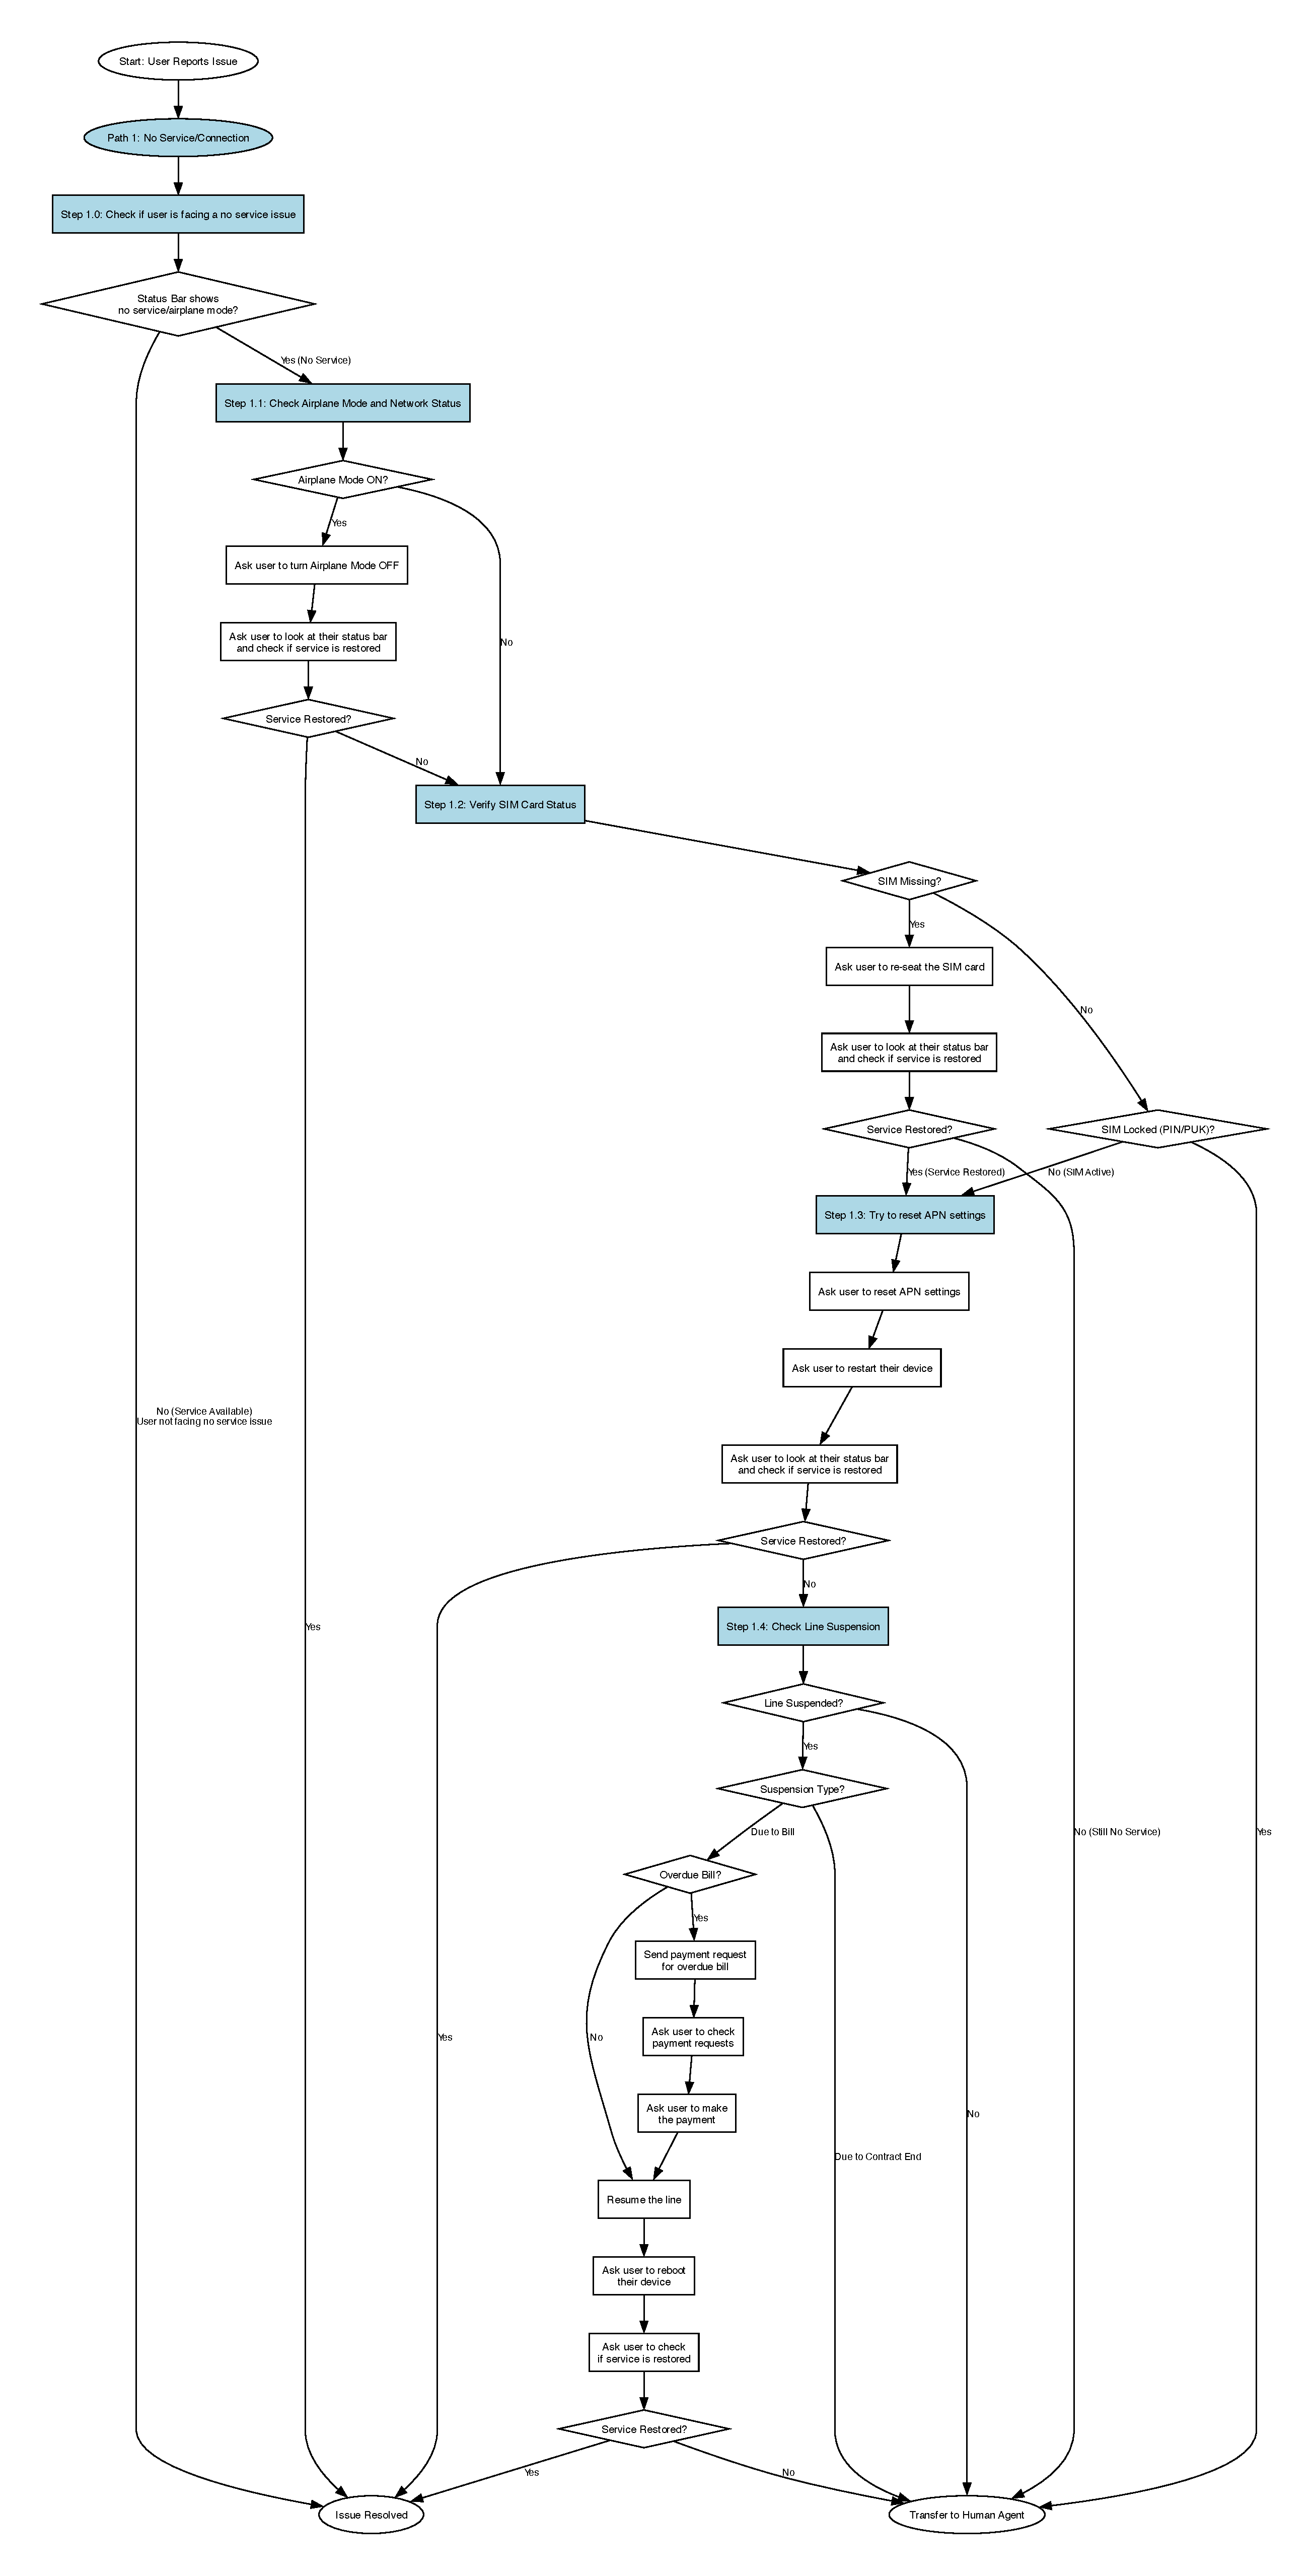
\includegraphics[width=0.7\textwidth]{figures/workflows/tech_support_path1_no_service.pdf}
    \caption{Troubleshooting workflow for \serviceissue}
    \label{fig:workflow-no-service}
\end{figure}

\begin{figure}[htbp]
    \centering
    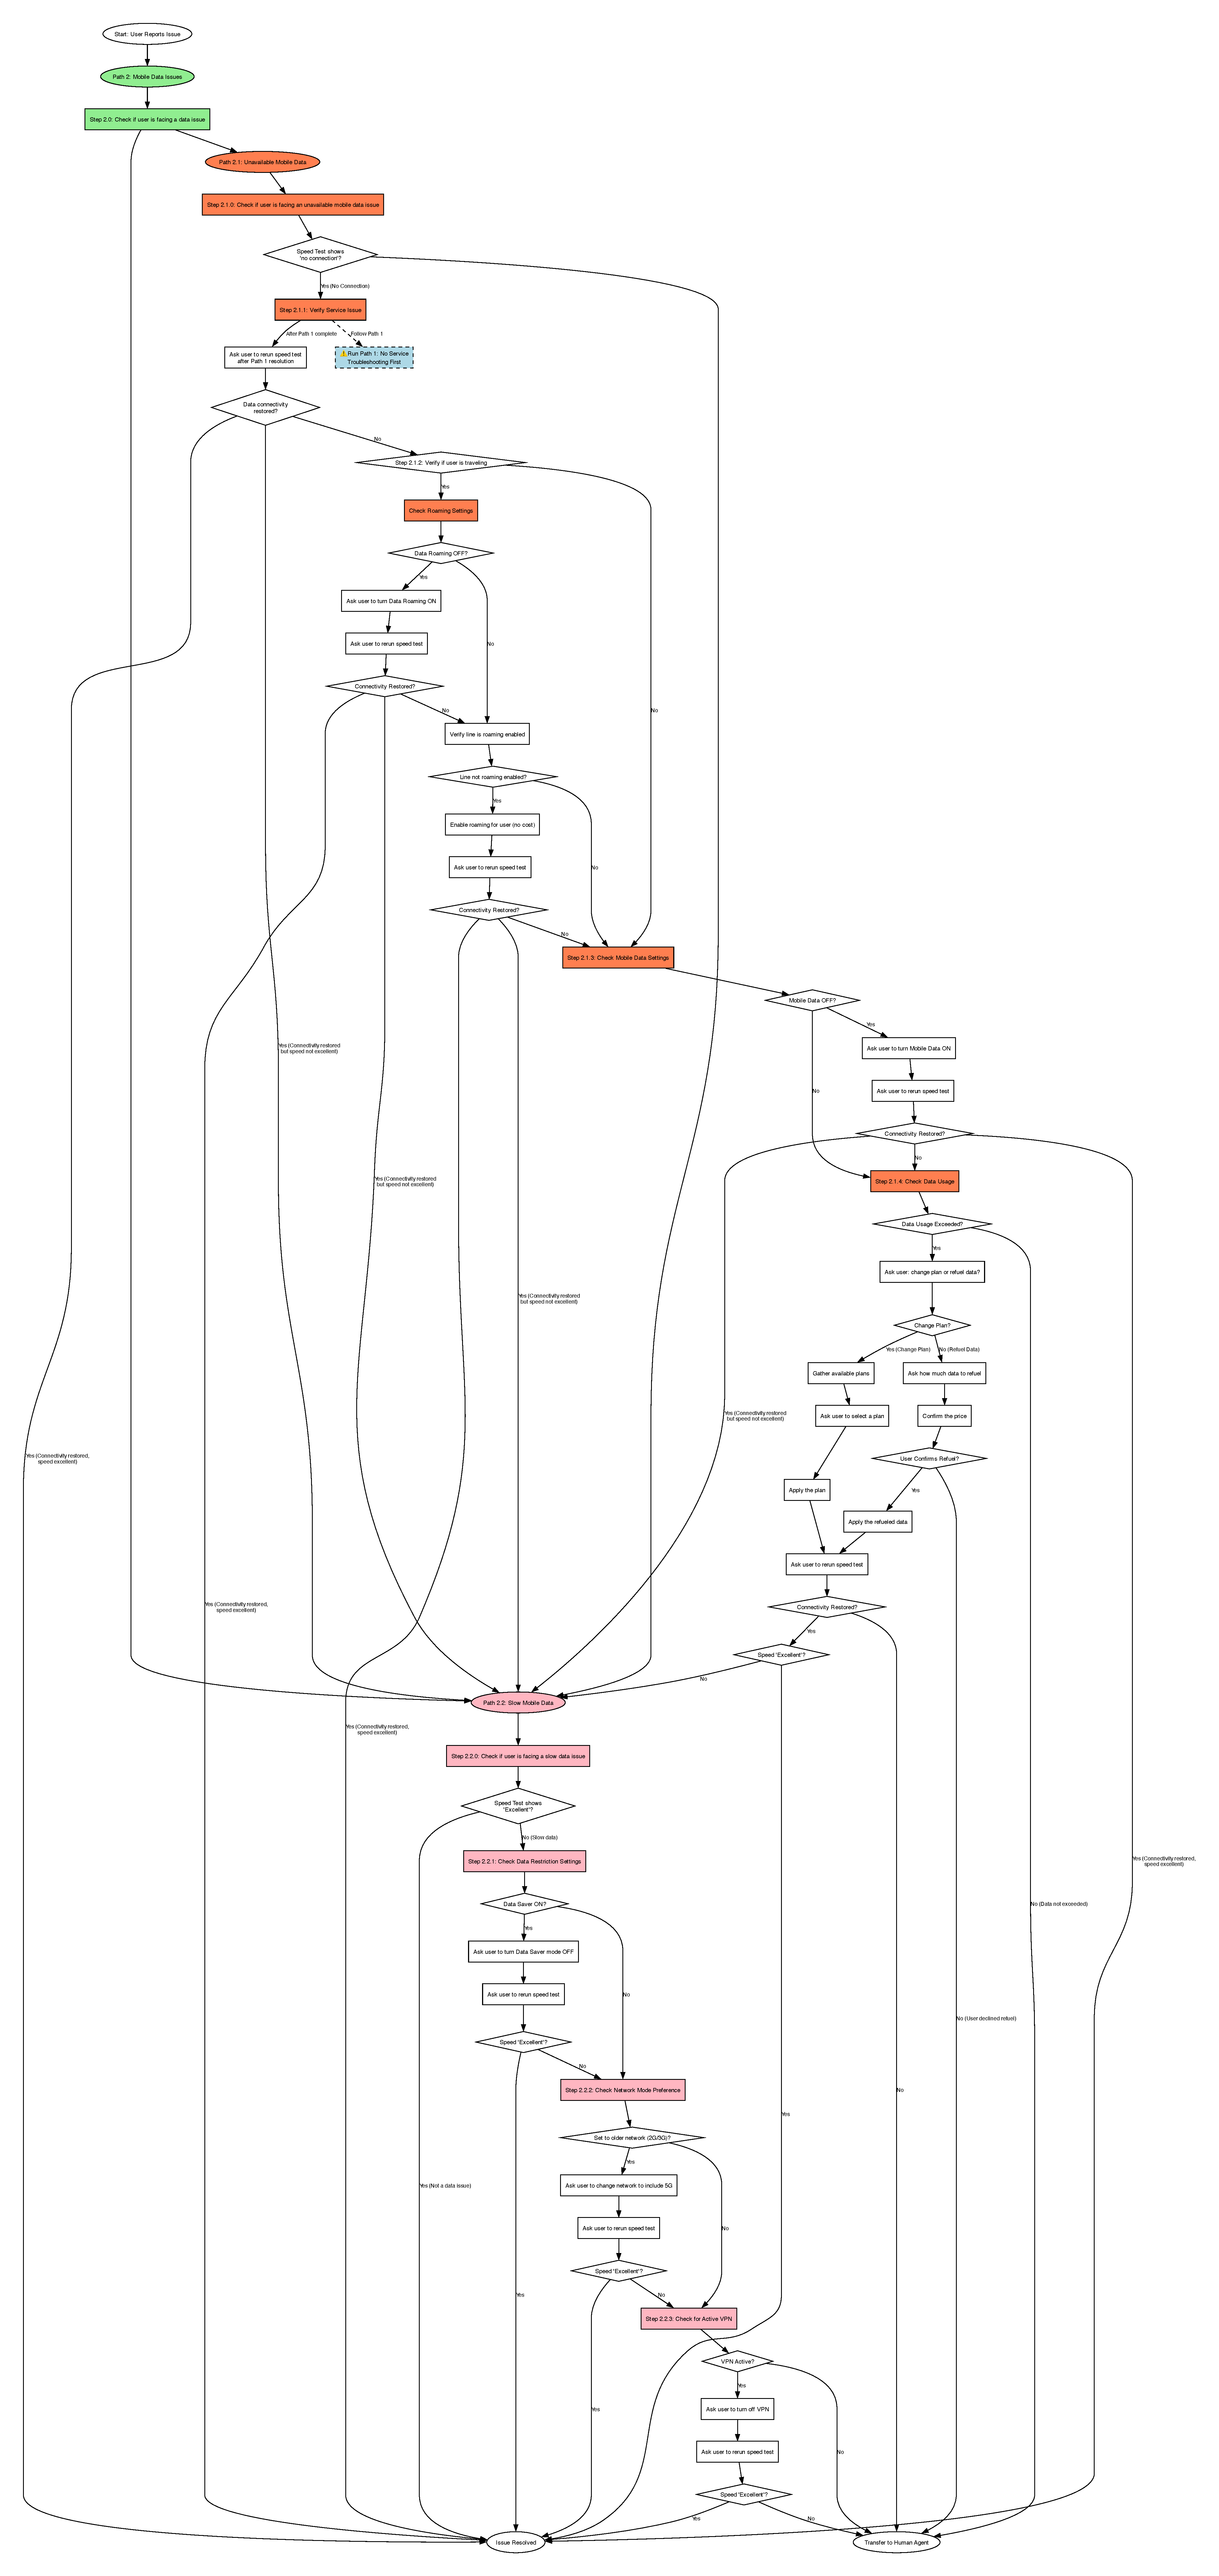
\includegraphics[width=0.7\textwidth]{figures/workflows/tech_support_path2_mobile_data.pdf}
    \caption{Troubleshooting workflow for \mobiledataissue}
    \label{fig:workflow-mobile-data}
\end{figure}

\begin{figure}[htbp]
    \centering
    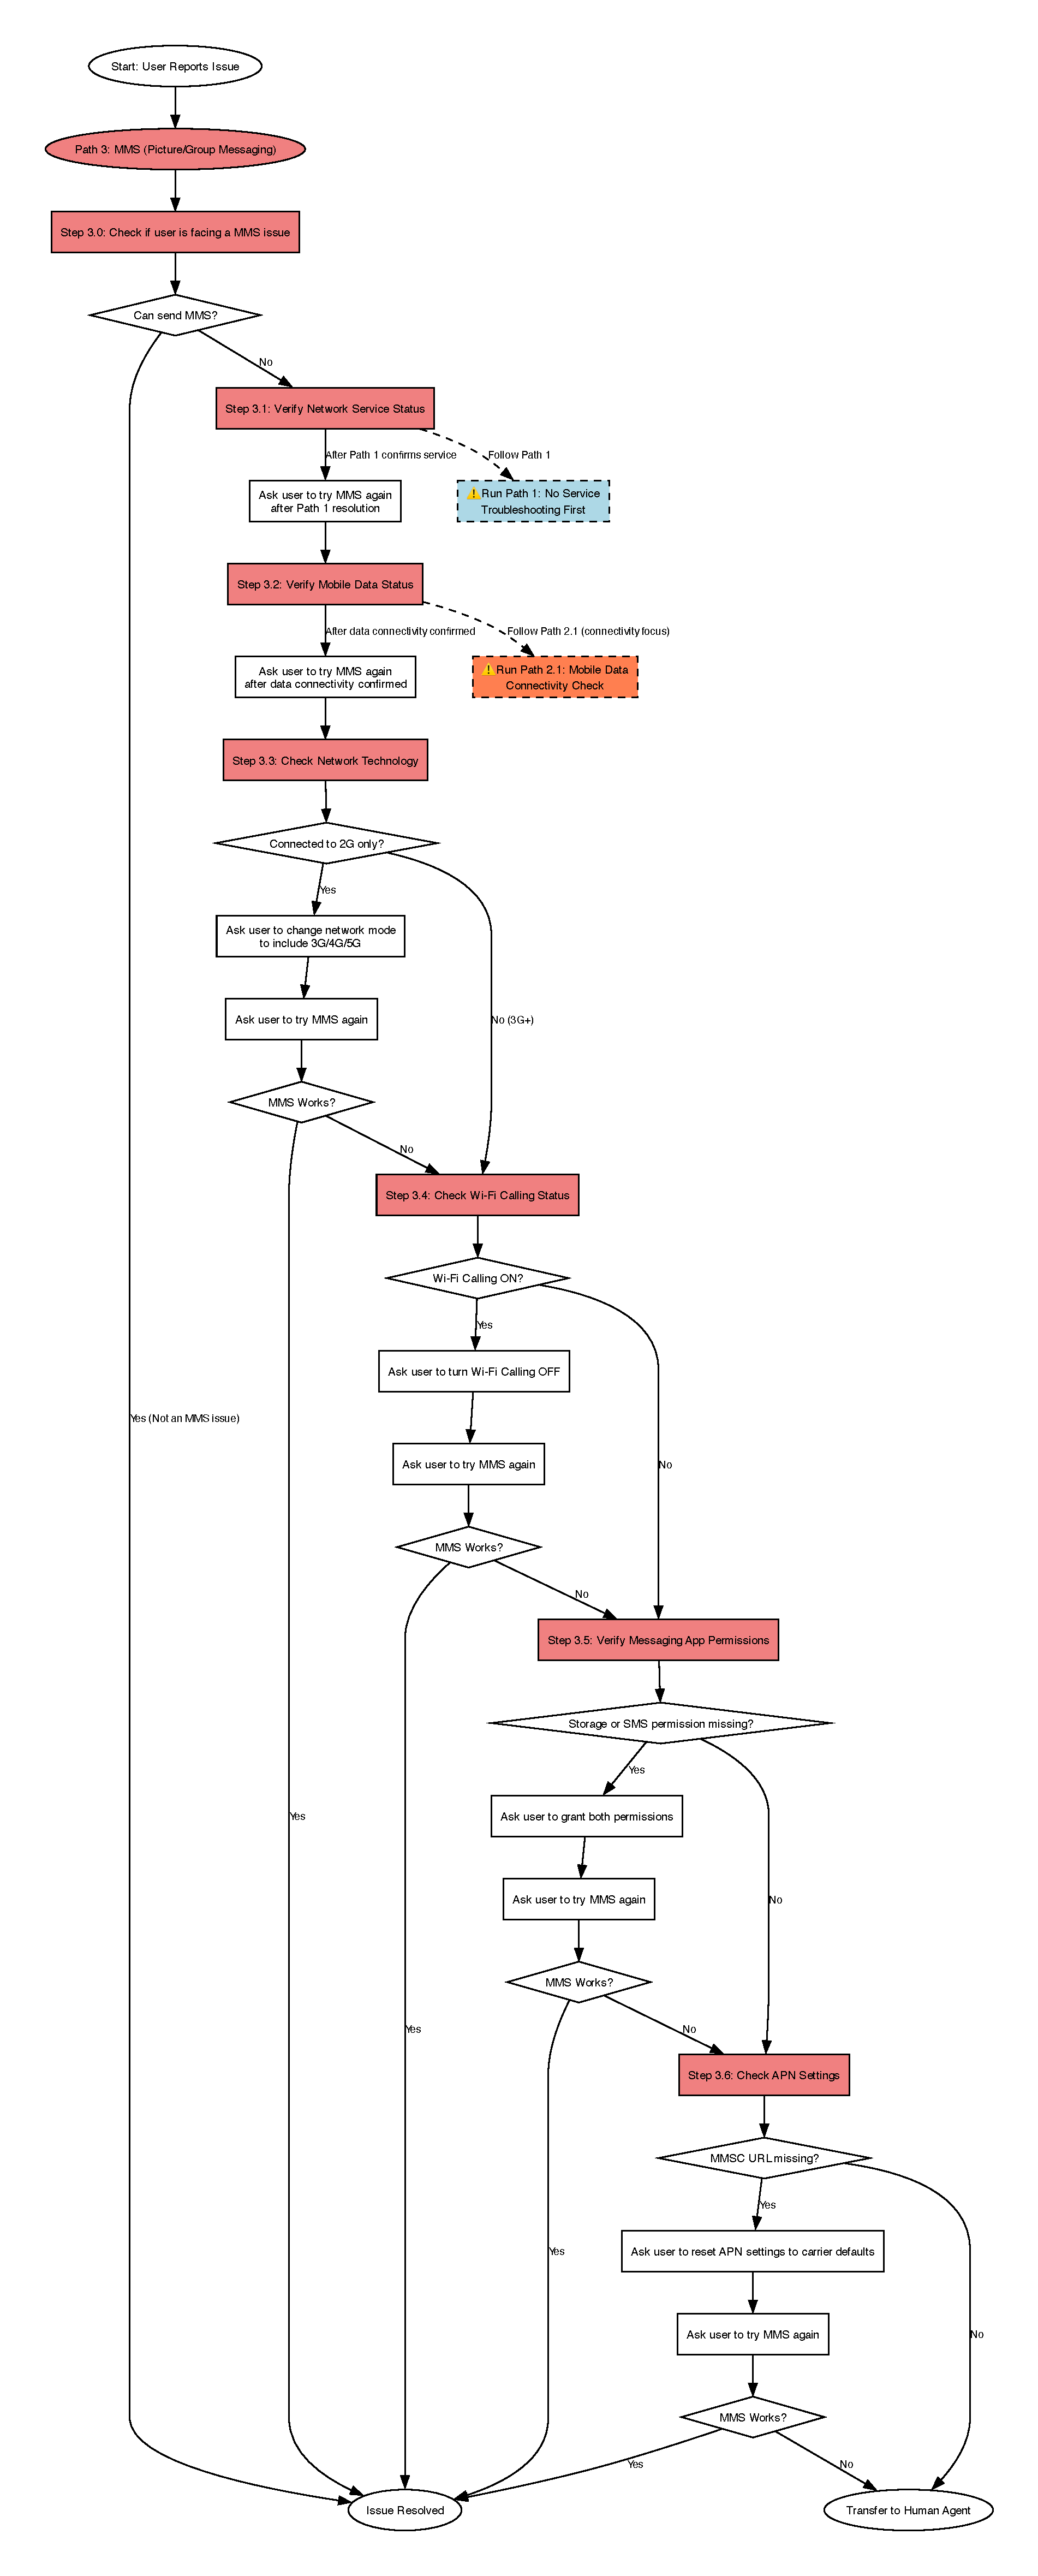
\includegraphics[width=0.7\textwidth]{figures/workflows/tech_support_path3_mms.pdf}
    \caption{Troubleshooting workflow for \mmsissue}
    \label{fig:workflow-mms}
\end{figure}
